\documentclass[times, 10pt,twocolumn]{article} 
\usepackage{latex8}
\usepackage{times}
\usepackage{xspace}
\usepackage{graphicx}
\usepackage{float}
\usepackage{comment}
\newcommand{\igH}[1]{\includegraphics[height=.9\textheight]{#1}}
\newcommand{\igHF}[1]{\includegraphics[height=\textheight]{#1}}
\newcommand{\igHhalf}[1]{\includegraphics[height=.4\textheight]{#1}}
\newcommand{\igHs}[1]{\includegraphics[height=.3\textheight]{#1}}
\newcommand{\igHthird}[1]{\includegraphics[height=.32\textheight]{#1}}
\newcommand{\igHh}[1]{\includegraphics[height=.45\textheight]{#1}}
\newcommand{\igW}[1]{\includegraphics[width=.9\textwidth]{#1}}
\newcommand{\igWh}[1]{\includegraphics[width=.5\textwidth]{#1}}
\newcommand{\igWhs}[1]{\includegraphics[width=.45\textwidth]{#1}}
\newcommand{\igWhh}[1]{\includegraphics[width=.7\textwidth]{#1}}
\newcommand{\igWhalf}[1]{\includegraphics[width=.5\textwidth]{#1}}
\newcommand{\igWs}[1]{\includegraphics[width=.3\textwidth]{#1}}
\newcommand{\igWF}[1]{\includegraphics[width=\textwidth]{#1}}

\newcommand{\histodiff}{\emph{HistODiff}\xspace}
\newcommand{\crex}{\emph{C-REX}\xspace}
\newcommand{\loggen}{\emph{LogGen}\xspace}

\newcommand{\yarn}{\emph{YARN\xspace}}
\newcommand{\evoflash}{\yarn}
\newcommand{\YARN}{\yarn}
\newcommand{\postgresql}{\emph{PostgreSQL}\xspace}
\newcommand{\cvsup}{\emph{CVSup}\xspace}
\newcommand{\Subsection}[1]{\subsection{#1}}

\newcommand{\shtn}{\vspace*{-.5em}}

%TODO:
% Edit 
% Make 9 pages


%\documentstyle[times,art10,twocolumn,latex8]{article}

%------------------------------------------------------------------------- 
% take the % away on next line to produce the final camera-ready version 
\pagestyle{empty}

%------------------------------------------------------------------------- 

\begin{comment}

TODO:
DROP TO 8 PAGES
EDIT
ENSURE ANIMATION


XXX EDIT XXX


+ Intro good but still needs work and gets on track
+ Flip book is cool
X MOTIVATION is unclear
? Rewrite necessary?
? in the case study we do not see from the balls the information we see
? No one cares about the tool chain
? related work should be on top - what?
- So the question is what kind of insights somebody can get looking such balls? or what is the purpose of the balls? to what usage do you intend them? 
- move problem section is in the discussion
- section 3 needs an example 
- section 3 given different choices, why do you use them? - unclear
- eval different presentations

X CREX limitations (not OO)
X References are missing dates 1, 2, 10 
X intro lacks references and is aimless: please choose between a summary of your approach or a description of existings tools along with their drawbacks... 
X why yarn, why flipbook none of what is shown uses yarn
X Maletic et al does not animate
X case study needs to link the visualization to the article
X Figure 4 doesn't show the util - sys control manager
X 2 figures are useless (at the back)
X no one cares about postgresql architecture
X Visual walk through should discuss the subsystems
X section 4 (case study) talk more about the figure than postgresql


what do yarn balls show us? messiness of architecture

\end{comment}


\begin{document}
\newcommand{\names}{Abram Hindle, Zhen Ming Jiang, Walid Koleilat,
  Michael W. Godfrey, Richard C. Holt}
\author{
\names \\
University of Waterloo and University of Victoria\\
ahindle@cs.uwaterloo.ca, zmjiang@ece.uvic.ca, \{wkoleila,migod,holt\}@cs.uwaterloo.ca
}
\title{
YARN: Animating Software Evolution
}

\maketitle
\thispagestyle{empty}

\begin{abstract}

  A problem that faces the study of software evolution is how to
  explore the aggregated and cumulative effects of changes that occur
  within a software system over time.  In this paper we describe an
  approach to modeling, extracting, and animating the architectural
  evolution of a software system.  We have built a prototype tool
  called \YARN (Yet Another Reverse-engineering Narrative) that
  implements our approach; \YARN mines the source code changes of the
  target system, and generates \YARN ``balls'' (animations) that a
  viewer can unravel (watch).  The animation is based on a static
  layout of the modules connected by animated edges that model the
  changing dependencies.  The edges can be weighted by the number of
  dependencies or the importance of the change.  We demonstrate our
  approach by visualizing the evolution of \postgresql DBMS.

\end{abstract}

\shtn
\Section{Introduction}
\shtn

\newcommand{\abram}[1]{\emph{(***ABRAM***: #1)}}
\newcommand{\graphfigfile}[1]{presentation/graph#1}
\newcommand{\graphlabel}[1]{fig:graph#1}
\newcommand{\yarnshots}{6}
\newcommand{\graphfig}[1]{
\begin{figure}[!b]
  \centering
  \igWh{\graphfigfile{#1}}
  \caption{\postgresql \YARN Flip-book shot #1/\yarnshots}
  \label{\graphlabel{#1}}
\end{figure}
}



Successful software systems evolve in many ways and for many reasons:
bugs are found and fixed, new features and deployment environments are
requested by users, and systems are refactored by developers to
improve the internal design.  Successful software systems that grow in
size and complexity over many years present a challenge to their
maintainers: how can these systems best be modelled, visualized, and
ultimately understood given the amount of detail present and the
volume of change.

For a given system, a developer may have access to static
``snapshots'' of its software architecture and its internal
dependencies.  These snapshots may be hand-drawn by an expert or
automatically extracted from the source code.  However, in practice
these approaches are not well suited to the task of understanding how
the system has evolved. Hand drawn snapshots are often not maintained
as the system ages, and automated architecture visualization tools
tend to emphasize a static view of the current version of the system.

Emphasizing the changes to a system's architecture requires refocusing
the supporting tools toward calculating architectural deltas and then
representing them effectively to the user.  Thus software architecture
needs to be extracted incrementally to reflect the historical changes.
In our case, we establish a baseline architecture for the system, and
then examine the CVS commits that contain the code for the changes.
After analyzing the results and reconciling the changes against the
baseline, the resulting architectural model of the system and its
changes can be presented using an animated visualization.

Animating the changes is an intuitive and natural way to compare
changes visually over time.  We start by showing the state of the
architectural dependencies within the system at a chosen baseline
version, and then show the user the subsequent changes progressively
as animations of the changing architectural visual model.  Change can
be shown cumulatively.  Cumulative views allow us to compare instances
sequentially, this helps us to compare the dependencies at two
different points in time, and animate the transition.



%This is
%often a problem with existing extractors because they may provide only only
%a snapshot of a change and are not necessarily easy to reconcile to the
%state of the system.


%Tools to aid in studying the evolution of software systems typically deal
%with very large data sets; often the data sets are so large that it is
%impossible or impractical to view all of the data at once. 

The set of data we analyze is often quite large and is difficult to
represent all at once in a way that is both meaningful and useful.
Animation enables us to traverse this rich and large information space
and interpret the data visually rather than in a textual or
statistical way.

Keeping the positions of the nodes fixed encourages the user to create
a stable mental model of the system's structure, allowing the user to
concentrate on the interactions between changing dependencies over
time and to observe the interactions between the system's components.
Animation exploits the temporality of the data in the repository and
helps to illustrate the dynamic behavior of the evolving dependencies
between modules.  We employ two approaches to represent the
dependencies: the cumulative addition of dependencies and the
difference of edge weights between changes.

%RCH - OMIT OR CLEAR UP (SEE WALID)
% Our motivation was that we would like to visualize the architecture
% at each revision. We had some idea of what the changes would
% look like, but in a textual form the differences were not obvious.
% There was so much data it was hard to interpret without some
% abstraction or visualization. As well we found that it was difficult
% to communicate what we saw to others. We wanted to be able to share
% our results with others to show them what we saw without having to do
% the same extraction. We hope this animation will better illustrate the
% change in coupling over time between modules, and elaborate on
% developers' mental models of software \cite{holt02software}.

Our tool, \YARN (Yet Another Reverse-engineering Narrative), generates
animations of the changing dependencies (edges) between subsystems
(vertices) of a project.  These changes are animated via
varying edge width and edge color, against statically placed vertices
which represent subsystems of the project being studied. Figure
\ref{fig:evoscreen} provides an annotated look at a \yarn ball
produced based on \postgresql.

Our primary motivation behind \YARN was that we wanted to visualize
the changing architecture and share these visualizations with others.
We wanted to convey our mental model of the
software\cite{holt02software} via modular decomposition, yet we had to
deal with a large amount of data which was hard to interpret in text
form.  \YARN balls help us visualize change and share these
visualizations with others.  \YARN balls could be useful for managers
or newcomers just to summarize the concrete architectural state of a
project, or show how the project has evolved.

In this paper, we describe our approach to extracting, modeling, and
animating architectural evolution, as implemented in our tool \YARN.
We have included an example use of \YARN on \postgresql and its
generated \YARN Ball animations in a flip-book-like form (figures
\ref{fig:graph1}, \ref{fig:graph2}, \ref{fig:graph3},
\ref{fig:graph4}, \ref{fig:graph5}, \ref{fig:graph6}); thus, the
reader can manually animate the printed YARN Ball like a flip-book.





\shtn
\Section{Related Research}
\shtn

One of the earliest uses of program visualization and animation is the
well known film ``Sorting Out Sorting'' by Baecker et
al.~\cite{sortingout}, which animated how values can be sorted by
various algorithms.  More recently, Gall et al. used 3D graphics to
compare releases of a project side by side \cite{GallJR99}.  Marcus et
al. have also used 3D visualization of source code \cite{maletic}.
%Telea et al.~\cite{} used animation for
%interactivity rather than to represent time.  
Mesnage et al.~\cite{DBLP:conf/vissoft/MesnageL05} created web
embeddable presentations of software evolution matrices using VRML.
Beyer et al.~\cite{storyboard} used animation and software evolution
metrics to storyboard changes to files. Evograph maps time to
timelines rather than animations \cite{DBLP:conf/wcre/FischerG06} yet
uses architectural fact extraction similar to \crex and
\histodiff.

Lungu et al. \cite{lungu} produced film strips which were similar to
our flip book approach in this paper.  D'Abrmos et al.
\cite{DBLP:conf/wcre/DAmbrosL06} produced a series of radar plots
which used distance from the center of a visualization, instead of
edge width, (like a radar display) as an indicator of coupling. Many
of these visualization
tools~\cite{lungu,DBLP:conf/wcre/DAmbrosL06,pinzger-softvis05,ratzinger-iwpse05,DBLP:conf/vissoft/TeleaV05},
which display graphs of modules and their coupling metrics as edges,
implement animation interactively rather than as a free
playing animation like \yarn.




Our architectural views are similar to those of Rigi \cite{rigi} and
Shrimp \cite{shrimp}. Shrimps uses animation to support iterative
navigation instead of representing change over time.  
Finally, we note that 
our architectural model of \postgresql was adapted from that of
Dong et al.~\cite{dong}.


\begin{comment}
Lungu et al. of CSMR 2007 - related because of film strip thus animation, inter module dependencies


M. Fischer and H. Gall, EvoGraph: A Lightweight Approach to
Evolutionary and Structural Analysis of Large Software Systems, WCRE '06 - crosscutting changes, similar fact extraction, differences is we use architecture, they just use directories, not animation, less static assumptions

M. D'Ambros and M. Lanza, Reverse Engineering with Logical Coupling, WCRE
'06 - time or age represented by distance to a focal point, coupling, iteractive animation with a slider. Radar view.

J. Ratzinger, M. Fischer, H. Gall, EvoLens: Lens-View Visualizations
of Evolution Data, IWPSE '05 - interactively animated, lens view, animating edges via color, non-animated but interactive, coupling, analysis process, metrics

M. Pinzger, H. Gall, M. Fischer and M.
Lanza, Visualizing Multiple Evolution Metrics, SoftVis '05 
Uses nodes and edge width, side by side comparison, multiple metrics, edge width


 T. Zimmermann and P. Weissgerber, Preprocessing CVS Data for
Fine-Grained Analysis, MSR '04 -- Oh come on we reference tonnes of MSR work why do we have to go back to the start?
\end{comment}


\shtn
\Section{Tools}
\shtn

\graphfig{1}

\emph{C-REX} is used to extract the architectural information from the
CVS repository of \postgresql.  Once extraction is done, we run
\emph{HistODiff} (part of \YARN), which makes use of \emph{C-REX}'s
output to compute the number of dependencies between subsystems,
output the dependency graph, and highlight architecturally important
changes.  \YARN reads these dependency graphs and then produces \YARN
Ball animations that can be played back by the user.
%Figure \ref{fig:approach} illustrates
%the extraction flow that we have used in our analysis.

\shtn
\Subsection{C-Rex}
\shtn

%XXX SHORTEN THIS

We use \emph{C-REX}~\cite{crex} as our fact extractor, as it has been
designed specifically for conducting historical architectural
analysis.  It has several advantages over most architectural fact
extractors.  First, traditional snapshot fact extractors, such as
\emph{LDX}~\cite{ldx}, \emph{RIGI}~\cite{rigi}, and
\emph{CPPX}~\cite{cppx}, are designed to retrieve architectural
information from only one version of a system.  \emph{C-REX} is an
evolutionary source code extractor; it extracts information from
version control systems and recovers architectural information over a
period of time.  Second, source code might not compile properly due to
the use of different programming language dialects, syntax errors,
etc.  In this situation, many parser-based extractors will fail, but
\emph{C-REX} avoids fully parsing the source code by making use of the
\emph{ctags} source code tokenizing tool.% \cite{ctags}.  
This makes
\emph{C-REX} more robust than most extractors.  Finally, most
extractors operate on the preprocessed code or the object code.
Because of compilation flags, a parser-based extraction results may
contain information specific to only a particular configuration;
\emph{C-REX} operates on the original source code, therefore it can
extract more information relevant to software evolution than
parser-based extractors.

\emph{C-REX} analyzes the main branch of a system's source code
repository.  \crex extracts all the changes from each revision and
groups revisions into transactions.  It outputs two types of
information: a \emph{Global Symbol Table} and a set of
\emph{Transaction Changes}\cite{zimmermann-msr-2004}.

The \emph{Global Symbol Table} maps all of the programming language
entities ever defined during the history of software development to
the file locations where these entities are defined.  An entity can be
of any C language type, such as a macro, variable, function, struct,
enum, etc.  \crex uses static analysis to keep track of entities.



\emph{Transaction Changes} list the entity changes committed by the
same author, at approximately the same commit time, with the same log
message.  It contains the author's name, a unique hash value to
identify this transaction, the commit time, and the log message as
well as detailed entity changes.  An entity change can be one of three
types depending on the scope of the entity: \emph{modified} if the
entity exists in both the previous and current system revision,
\emph{added} if it exists only in the current revision, or
\emph{removed} if it exists only in the previous revision.
\emph{HistODiff} uses these transactions to maintain its model of the
system.


Within each changed entity, \crex keeps tracks of changes in entity types,
dependencies, and comments.  If the entity is a function, \crex also
tracks changes in parameters and return types. 
%- CREX limitations (not OO)
%Unfortunately \crex is unaware of the actual types within a system and
%is thus not aware of virtual dispatch that is prevalent in many
%languages like C++ or Java. 
\crex's output is then processed by our
tool, HistODiff.



\shtn
\Subsection{HistODiff}
\shtn


HistODiff analyzes \crex output, and creates graphs for \YARN
to animate. HistODiff performs many tasks such as symbol mapping,
architectural mapping, lifting and filtering.

%  it associates symbols to files; it resolves
%references between changing architectures; it performs ``lifting'' of
%architectural information; it filters the observed changes using heuristics
%to identify key changes; it produces graphs for viewing; and it creates
%reports of changes that are deemed interesting.  


\emph{Symbol Mapping:} \crex's output consists of many identifiers and
symbols per transaction, \histodiff resolves these symbols and
identifiers to functions and macros.

\emph{Architectural Mapping:} \crex produces a list of transactions
where entities such as functions, macros, and variables are added,
removed, and modified. \histodiff maps these transactions to
architectural entities. These transactions are used to update the
architectural dependency graph per each commit.

%XXX Abstracting?
\emph{Lifting:} The change information is ``lifted'' to the
architectural level, where the top-level subsystems and their
dependencies are modeled.  Two kinds of graphs can be produced: a
dependency graph between subsystems over time, and a difference graph
that shows the dependency changes between subsystems before and after
a given transaction.  The graphs have directed weighted edges that
indicate the number of calls between modules.  It makes the assumption
that each file is associated with a single module within the module
hierarchy for the entire animation.

\emph{Filtering:} In large projects such as \postgresql there are a
very large number of changes to consider, but not all are
architecturally significant.  Large change transactions are noticeable
because they affect many files or have a large line count, but small
changes of one or two lines can also drastically alter the
architecture and change the dependencies between modules.  These are
important changes to make note of, because they could indicate some
kind of architectural rule violation or an important feature addition.

Our filtering heuristics retain transactions that affect the number
of dependencies between the top level subsystems that satisfy one or
more of the following criteria:

\begin{itemize}
\shtn
\item 
%$\bullet$
 The transaction adds a dependency between two subsystems that were 
    previously unconnected.

%$\bullet$ 
\item 
The transaction removes a dependency between two subsystems that
    causes them to be unconnected.

%$\bullet$
\item 
The transaction doubles the number of dependencies between two subsystems.

%$\bullet$
\item 
The transaction reduces the number of dependencies between two
    subsystems by half.
\shtn
\end{itemize}


\shtn
\Subsection{YARN}
\shtn

\graphfig{2}

%XXX - section 3 needs an example 
%XXX - section 3 given different choices, why do you use them? - unclear
%XXX - Eval different presentations

% We need evaluation of the visualization techniques

\begin{figure}[htb]
  \centering
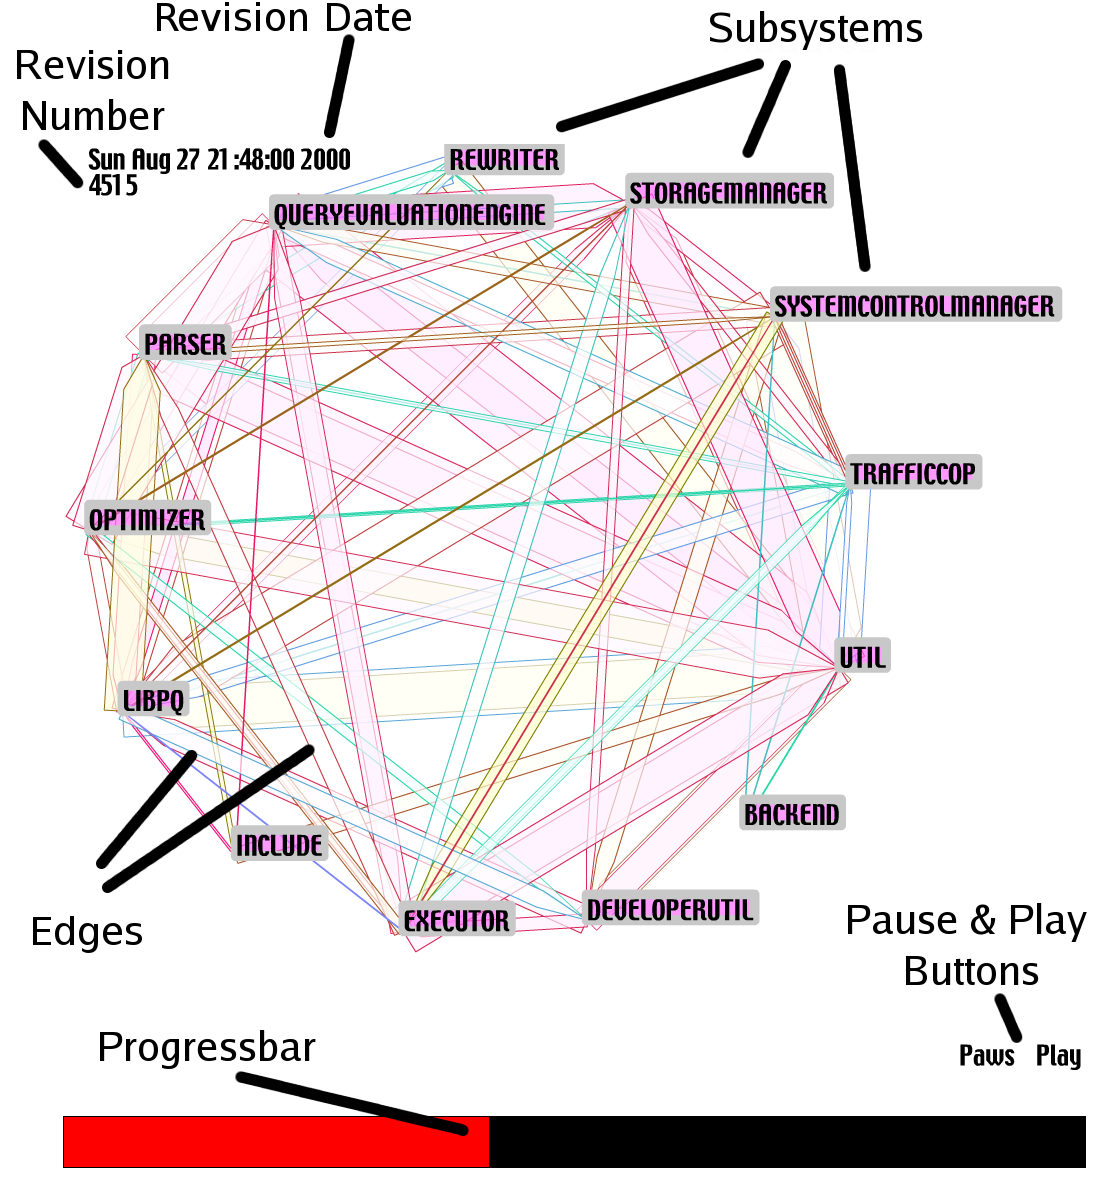
\includegraphics[width=.5\textwidth]{evoflash}
\caption{Screen-shot of \YARN with \postgresql}
\label{fig:evoscreen}
\end{figure}

The goal of \yarn (Yet Another Reverse-engineering Narrative) is to
provide a narrative animation; that is, the story of the evolution of
a software project over time.  \yarn uses \emph{HistODiff} output along with
some animation parameters to generate \yarn Balls
(animations), which can be unraveled (watched) by the user, in order
to learn about the history of the system's architecturally significant
changes.

\yarn uses \histodiff's graph output to create a graphical animation
of the architectural changes of a system. In the animation, the
thickness of the edges represents how many dependencies exist between
two modules.
%, we use the
%function $log^2(weight(u,v,t))$ to determine the edge's thickness
%based on its weight at a certain time.  
In figures \ref{fig:graph1} through \ref{fig:graph6}, we can see the
modules do not change position. They are laid out in a radial pattern
due to the high coupling and ease of layout.



Edges are directed; when displayed, the edge of lesser weight is shown
inside of the edge going in the reverse direction.  Edges are also rendered
transparently, thus intersections of edges are both visible and visually
resolvable.

\YARN animates edges in different ways:

\newcommand{\hilight}[1]{\textbf{#1}}

\hilight{Cumulative view:} Edges are shown the entire time when there
is a dependency between two modules. This approach emphasizes the current
state of the system and what edges have been changed.

\hilight{Delta view:} Edges are shown only when they change.  This
approach emphasizes what the actual changes are by removing the extra
information.

All of the the following algorithms assume that the edges are growing
and shrinking in width and that the nodes remain stationary while the
edges are being animated.

\YARN supports several coloring schemes. Each uses color in a different way,
in the animation, to emphasize certain aspect of the changes over time.
Three of these schemes are:



\label{sec:coloring}


\hilight{Color Changes on Modification:} This algorithm changes the
color of the edges, each time the edge is modified. This serves to
emphasize edges that change.  Per each revision a new color is
assigned. This color changes gradually over time.  When dependencies
between two modules change, the edge is highlighted with the current
color. This means edges that change frequently will flash with color.
Frequent edges will be colored similarly while edges which are
infrequently changed will have out-dated colors.  In figure
\ref{fig:evoscreen} we can see this algorithm in use, the edges that
have a similar color were changed at the same time, where as edges
with distinct colors have not been changed recently.  This
coloring scheme can be ambiguous; based on the colors chosen,
edges getting brighter or darker might suggest decay rather than
change to a user.  The suggested use for this algorithm is to emphasize
the rate of change and show all of the modifications that are occurring.



\graphfig{3}
\hilight{Highlight and Decay:} Each edge that is modified is
highlighted when a change occurs. It is highlighted by changing the
color to a bright bold color; then over the period of a few changes
the color of that edge decays back down to a neutral color. This color
function emphasizes recent changes. The flip book figures
(\ref{fig:graph1}) uses this method.  Possible disadvantages are
that the decaying colors could look like new changes, also selecting
an appropriate decay time could be difficult depending on how busy the
graph is. Highlight and decay emphasize new changes, as old changes
disappear rapidly, it makes the current change more obvious by making
the past fade away.


\hilight{Highlight the Important Changes:} This coloring algorithm is
much like the highlight and decay algorithm except only the important
changes are highlighted instead of just the new changes.  Our
algorithm has designated certain changes as important based on our
importance metric.  The flip book figures (\ref{fig:graph1}) are
similar to this method.  This algorithm is
useful for highlighting changes that are flagged as important as it
demonstrates how the frequency of ``important'' changes.


Edge widths can be displayed in several different ways:


\hilight{Cumulative Width:} This edge width function is a scaling
function such as $log(weight(t,u,v))^2$ (where $u$ and $v$ are modules
and $weight(t,u,v)$ is the number of dependencies from $u$ to $v$ at
the current step $t$). Cumulative Width shows how many dependencies
currently exist between the two different modules. This scheme is
useful as it shows the current state of the architecture. This
algorithm shows the accumulation of dependencies up to the current
time.


%\item[Decaying Edge Width:] 
\hilight{Decaying Edge Width:} The older an edge gets the thinner it
gets.  Over time an edge shrinks (decays) until it reaches a minimum
width. When a change occurs, the edge gets thicker again. This scheme
emphasizes the current change over the past changes, it doesn't allow
for much historical comparison and can unnecessarily indicate a
decreasing relationship, but serves to highlight the content of the
revision.

%\item[Edge Width as Age:] 
\hilight{Edge Width as Age:} Instead of the number of dependencies,
edge width indicates when the last change happened to the dependencies
between modules. This scheme reflects the frequency of change in
dependencies between two modules by the edge width itself. This can be
used to emphasize the dependencies that are frequently added.

%\end{description}
%RCH BAD NAME?
\shtn
\Subsection{Implementation}
\shtn

The animated changes are transactions. One frame represents one
transaction; \postgresql had over 10,800 frames of animation.  In the
top corner, the current date of the transaction is shown; see figure
\ref{fig:evoscreen}.  Underneath is the order of the revision. At the
bottom, a time-line shows relatively when the transaction occurs.
The time-line is interactive, it allows jumping to any part of the
evolution of the project. 
%The ``Paws'' (a reference to cats and
%yarn) and play buttons pause and play the animation.

The animations are created in SWF (Macromedia Flash) format using
vector graphics, and can be embedded into web-pages and viewed by most
modern browsers.  This could be used in hypermedia software evolution
systems such as the Software Bookshelf \cite{pbs} or SoftChange
\cite{dmgseke2004}.

Modules can be laid out manually or automatically. Automatic layout
algorithms currently include radial or matrix layouts. The radial
layout is useful for systems like \postgresql, where there are many
dependencies.

Figures \ref{fig:graph1}, \ref{fig:graph2}, \ref{fig:graph3},
\ref{fig:graph4}, \ref{fig:graph5}, and \ref{fig:graph6} depict 6
frames from a \yarn ball of \postgresql (cropped) using the Highlight
and Decay color function and the Cumulative Width edge function.
Figure \ref{fig:evoscreen} depicts a screen-shot of \yarn in action.

\shtn
\Section{Exploratory Case Study of \postgresql}
\shtn

\graphfig{4}

%XXX SIMPLIFY ARCHITECTURE
%\shtn
%\Subsection{Architecture}
%\shtn

\postgresql is a well known open source DBMS that is in wide use.
\postgresql has a well defined layered architecture.
%(Fig.\
%\ref{fig:architecture}).  
%The use of layering provides many advantages including the separation
%of concerns and abstraction.  
The three layers are:

\hilight{Client Interface Layer:} This layer accepts input from the
users through a variety of user interfaces.  It submits the queries to
the Backend layer below and returns the answers.

\hilight{Backend:} This layer parses the user's query, expands it, and
presents it to the optimizer which uses information to produce the
most efficient execution plan for the evaluation.  In order to execute
the plan tree, this layer uses the I/O functions in the Data Store
Layer.

\hilight{Data Store Layer:} This layer deals with managing space on
disk, where the data is stored.  Upper layers require this layer to
write or read pages.





Using figure \ref{fig:graph4} going clockwise we'll describe the sub modules of the layers:

%YES
\hilight{Rewriter:} is the primary module for the rewriting queries which
      are recursive or can be optimized.

%YES
\hilight{Storage Manager:} is found inside of the data layer, it manages files
      and pages of the database.

%YES
\hilight{System Control Manager:} handles authentication and starts and stops
       \texttt{postgres} processes.

%YES
\hilight{Traffic Cop:} handles the flow control of queries.

%YES
\hilight{Util:} consists of utility procedures and routines that different
       modules use to do their jobs, especially Backend.
%WHAT

\hilight{Backend:} is a small module which stitches together
       the various modules to create the \postgresql server.

%WHAT DEVELOPERUTIL
\hilight{Developer Util:} consists of code which end-users will probably not use, like the test suite.

%YES
\hilight{Executor:} executes the query plan (execution tree).

%WHAT
\hilight{Include:} consists of common include files shared amongst
many modules, particularly those which use Util.

%YES
\hilight{LibPQ:} enables the client or user to query the RDBMS.

%YES
\hilight{Optimizer:} attempts to choose an optimal query plan structure for a
      given query.

%YES
\hilight{Parser:} tokenizes and parses SQL queries.


%WHAT 
\hilight{Query Evaluation Engine:} consists of submodules (Catalog,
Command and Nodes) used to represent queries and meta-data about the
databases.

%\hilight{Command:} is a query which doesn't need the Optimizer.

%\hilight{Catalog:} is where the RDBMS stores the meta data, e.g information
%       about tables, columns, values etc.

%\hilight{Nodes:} are responsible for storing the queries in a specified common
%      data structure called Nodes Structure.




\shtn
\Subsection{Timeline of \postgresql}
\shtn

We examined the history of architectural changes of \postgresql by
manually inspecting a few architecturally significant transactions.
\histodiff flagged about 100 transactions that it considered to be
architecturally significant; that is, they have either added or
removed dependencies which have significantly increased or decreased
the degree of coupling between subsystems.

We divided the history, consisting of a sequence of transactions, into
three periods with an equal number of flagged changes.  The time
intervals of these periods varied considerably because the rate of
occurrence of changes varied.

%\begin{itemize}
%\item 
1996 to 1998: \postgresql was released as Open Source Software.
  Portability and reimplementation of features such as ODBC were
  included (see figures \ref{fig:graph1} and \ref{fig:graph2}).

%\item 
1998 to 2000: \postgresql was still in flux, ODBC updates
  occurred and \postgresql was extended by the PL/pgSQL language (see
  figures \ref{fig:graph3} and \ref{fig:graph4}).
    
%\item 
2000 to 2005: \postgresql was maintained, as a reasonably mature
  system.  Fewer features were added, more auditing and bug fixing occurred
  (see figures \ref{fig:graph5} and \ref{fig:graph6}).
%\end{itemize}


\begin{figure*}[ht]
  \centering
\begin{tabular}{lr}
    \igWhs{presentation/graph4} & \igWhs{analysis2005}\\
\end{tabular}
\caption{Important architectural changes done during the last 5
years} \label{fig:pgsql05}
\end{figure*}


Figure \ref{fig:pgsql05} depicts the changes made to the system
starting from 2001 to 2005; larger changes are highlighted. This was a
notable period for \postgresql where large changes to the source code
included new implementations of SQL statements, improving triggers,
JOINS and dropped columns. Most of the changes were maintenance and
improvement of properties such as robustness, security and
performance.  Security improvements %were spurred by problems found by
%``white hat hackers'', who found 
included fixing flaws related to interrupt handling
and critical sections.  

\shtn
\Section{Visual Story of PostgreSQL}
\shtn \graphfig{5} There were many significant changes from 1996 to
2005; we have shown a few and have provided screen-shots (from our
\YARN ball \cite{yarnball}) of the revisions.  These screen-shots help
highlight the progression of architectural dependencies over time in
\postgresql. As well, they highlight the architecturally significant
changes that occurred over time. We will now show screenshots at times
when important changes were flagged; when we investigated we looked at
a few revisions within a small time window around that change.

The first notable change (figure \ref{fig:graph1}), shows that
dependencies changed between Parser, Query Evaluation Engine,
Storage Manager, Traffic Cop and Utils.  Investigation into the
revisions revealed that this change was the reimplementation of the
ODBC driver by Insight, and it was highlighted because of the doubling of
dependencies between Parser and Utils.


The second notable change is from figure \ref{fig:graph2}.  We can see
that the two corresponding dependencies that changed during this time
are highlighted, namely those between the System Control Manager
and Util. Although \yarn does not tell the full story,
the revisions around this time revealed that
the embedded language PL/TCL was added.  PL/TCL is an extension to
\postgresql which allows the TCL programming language to be used in
stored procedures.


The added dependencies between Util and System Control Manager,
Parser, and Executor were the most notable in figure \ref{fig:graph3}
(color-enhanced).  By investigating the revisions, we found this was
the addition of the PL/PgSQL embedded language: a language for stored
procedures in \postgresql which wasn't TCL.  It is important and
noteworthy because the inclusion of the language crosscut multiple
modules and introduced more coupling.

The fourth change (figure \ref{fig:graph4}) we show is actually both
an increase and a reduction of coupling.  This change was highlighted
by our importance metric due to a reduction of dependencies.  It is
hard to see since we haven't shown the immediate preceding changes,
but the coupling of LibPQ to the System Control Manager has been
reduced. Most of the other changes seem to show an increase in
coupling. Investigation of the related revisions revealed that a
memory management submodule was rewritten, there were several bug
fixes and some dead code was removed.



From the fifth change (figure \ref{fig:graph5}), we see new coupling
from Include to Traffic-Cop, Include to LibPQ and LibPQ to Executor.
These changes were made to \postgresql due to the advice given by
``white hat hackers'' regarding security holes in the interrupt and
issues with some of the critical sections.

The sixth change (figure \ref{fig:graph6}) was important due to the
changes in dependencies that occurred between various modules and
LibPQ and Util.  The related revisions revealed that there was a
change to the Win32 signal-handling code. This change made signal
handling more portable via abstractions of the \texttt{kill} and
\texttt{sigsetmask} syscalls.

\shtn
\Section{Survey}
\shtn

In order to evaluate \yarn, we created an informal user survey to see
how intuitive the visualization was for users and if they were
interested in using \yarn.  The survey could be answered over email or
live over chat. Ten people took the survey, their backgrounds ranged
from high school Source Forge contributors, CS undergraduate students,
PhD students to full time developers. Most respondents answered all
the questions.

All users could use the functionality of a YARN Ball without much
difficulty. The navigation controls and the play and pause buttons
worked intuitively. Most users expected the pause animation on jump
feature.

Users did not know initially what the animation was about. They had to
be told it was about revisions to the source code and coupling. Some
users assumed this was the run time coupling until they were informed
otherwise.

Color-wise, most users like the highlight and decay based color schemes
where changes are highlighted in red and then slowly decay back to a
neutral color.

Users could infer coupling from the animation for changes with large
and small coupling. Generally users understood what the edge weights
meant.  Users did not seem to gain a better understanding of software
architecture. Due to a general lack of experience with PostgreSQL many
didn't have any expectations of the PostgreSQL architecture; one
respondent said they were not surprised since they had experience with
the architecture of the Linux kernel .

Some users said they would use the \yarn Balls if they were available
but were not actively going to create \yarn Balls.
Survey respondents suggested improvements such as making the
visualization 3D or projected onto a sphere, or the use of other
metrics.  Some said more data should be displayed like the change log
and a legend was needed.  Some suggested tweaking parameters like
color decay speed etc. One suggested coloring the edges to indicate
which module was being depended on.

\graphfig{6}

%XXX Not sure
%\Section{Discussion}

%* Did users use yarn balls as expected?
%* Were we succesful 
%* So the question is what kind of insights somebody can get looking such balls? or what is the purpose of the balls? to what usage do you intend them? %

%- move problem section is in the discussion
%- Visual limitations are not discussed




\shtn
\Section{Future Work}
\shtn

%* Layout
%* Interactivity
%* Hierarchy
%* Metrics

One extension to \YARN will be to its \YARN Ball user interface.  More
layout algorithms will be added to YARN.  We plan to add more
interactivity to the animation. This would include dragging and
dropping modules as well as expanding sub modules.  This would allow
hierarchical navigation of sub modules.  Different views of the
architecture are planned, such as a source control view which shows
which modules are coupled together per commit.  Other work includes
formally evaluating the use of animation for maintenance work and how
to improve scalability via lifting and new layouts.


\shtn
\Section{Conclusions}
\shtn

%NEEDS MORE WORK
%WHAT IS INTERESTING

In this paper, we have described an approach to extracting, modeling,
and animating architectural evolution of software systems, as
implemented in our prototype tool YARN.  The YARN tool aggregates this
data into animations, or YARN Balls, which can be explored by the user
to better understand the architectural evolution of the system under
study.  These YARN Balls can be embedded into web pages or shared in
order to communicate change based dependency information about
software projects.  Many different kinds of animations can be
produced.

The main contributions of this work include: an approach for
animating the evolution of a project's dependencies in a coherent
static manner; a system to view changes and the cumulative effects of
the changes; animations which provide a commit-level view of the
evolution of the project; and an informal user survey evaluating the
perception and usefulness of the visualization.

\shtn
\shtn
\subsubsection*{Acknowledgments} 
\shtn
Part of this research was funded
by an NSERC scholarship.

\begin{comment}

\begin{figure*}[p]
  \centering
  \igH{YARNApproach}
  \caption{Flow Control of Extraction with our tools}
  \label{fig:approach}
\end{figure*}

\begin{figure*}[p]
  \centering
    \igW{architecture}
\caption{Top Level Architecture of \postgresql}
\label{fig:architecture}
\end{figure*}

\end{comment}

\shtn

\bibliographystyle{latex8}

\shtn

\bibliography{msr-evoflash}

\end{document}
